\section{Suche nach neuer Physik}

In diesem letzten Versuchsteil soll nun innerhalb unserer Daten nach neuer Physik, genauer gesagt nach dem $Z'$-Boson gesucht werden.
Genauer wird nach einem $Z'$ gesucht, das in ein $t \overline{t}$ Paar zerfällt.
Dafür stehen wieder Monte-Carlo-Simulationen zur Verfügung, die solche Zerfälle für verschiedene Massen des $Z'$ im Bereich von 400 bis 3000 GeV simulieren.
Wie bei der Higgs-Analyse sollen dafür als erstes wieder Cuts implementiert werden.
Da dies völlig analog zur vorherigen Aufgabe geschah, werden wir auf Details dazu nicht groß eingehen und uns in dieser Auswertung vor allem auf die Ergebnisse der Cuts konzentrieren.
Im Abb.\ref{Cuts_z} sind beispielhaft die Impulse der Leptonen mit und ohne Cuts, sowie die invariante Masse dargestellt.
Hier ist zu beachten, dass die $Z'$-Ereignisse aufgrund ihrer geringen Häufigkeit um den Faktor 10 hervorgehoben wurden.
Wir können hier wieder Bereiche mit $Z'$-Ereignissen sehen.
Der Untergrund hier wird von $t \overline{t}$ Ereignissen dominiert.
Durch Auswahl unserer Cuts konnten der Untergrund wieder deutlich reduziert und die $Z'$ Ereignisse hervorgehoben werden.
Da wir für die Suche nach einem $Z' \rightarrow t \overline {t}$ Zerfall suchen, ist eine vollständige Beseitigung des $t$-Untergrundes nicht zu erwarten.
Im Bereich in dem die meisten $Z'$-Ereignisse zu erwarten sind, liegt das Verhältnis aus Daten und Untergrund wieder nahe 1, was für unsere Cuts spricht (siehe Abb. \ref{Cuts_z}.
Insbesondere bei der invarianten Masse sind die relativen Fehler hier jedoch recht hoch.
\begin{figure}[h]
\begin{subfigure}{.5\textwidth}
\centering
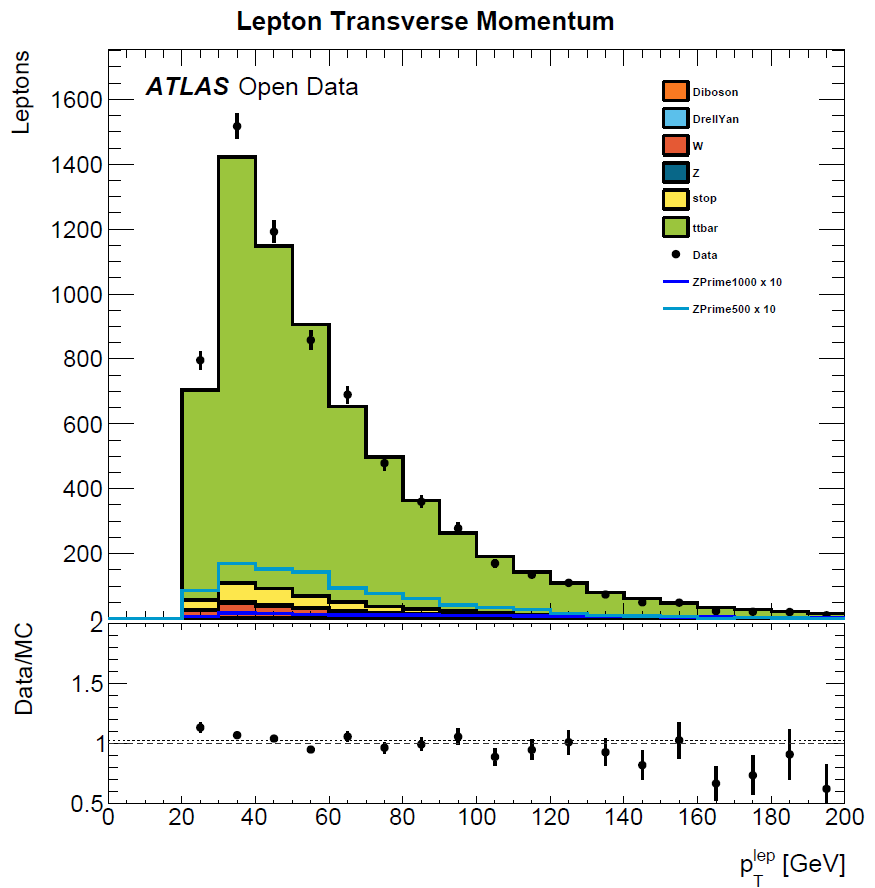
\includegraphics[width=.8\linewidth]{../Pictures/before.png}
\caption{Impulse ohne Cuts}
\end{subfigure}%
\begin{subfigure}{.5\textwidth}
\centering
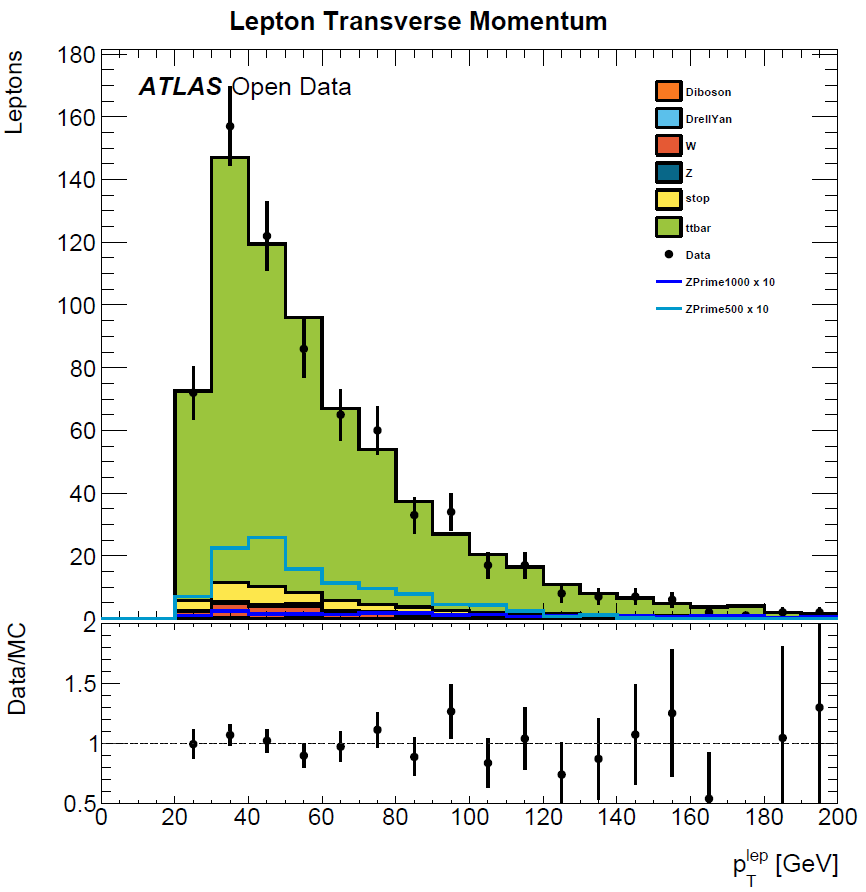
\includegraphics[width=.8\linewidth]{../Pictures/after.png}
\caption{Impulse mit Cuts}
\end{subfigure}%
\vskip\baselineskip
\begin{subfigure}{.5\textwidth}
\centering
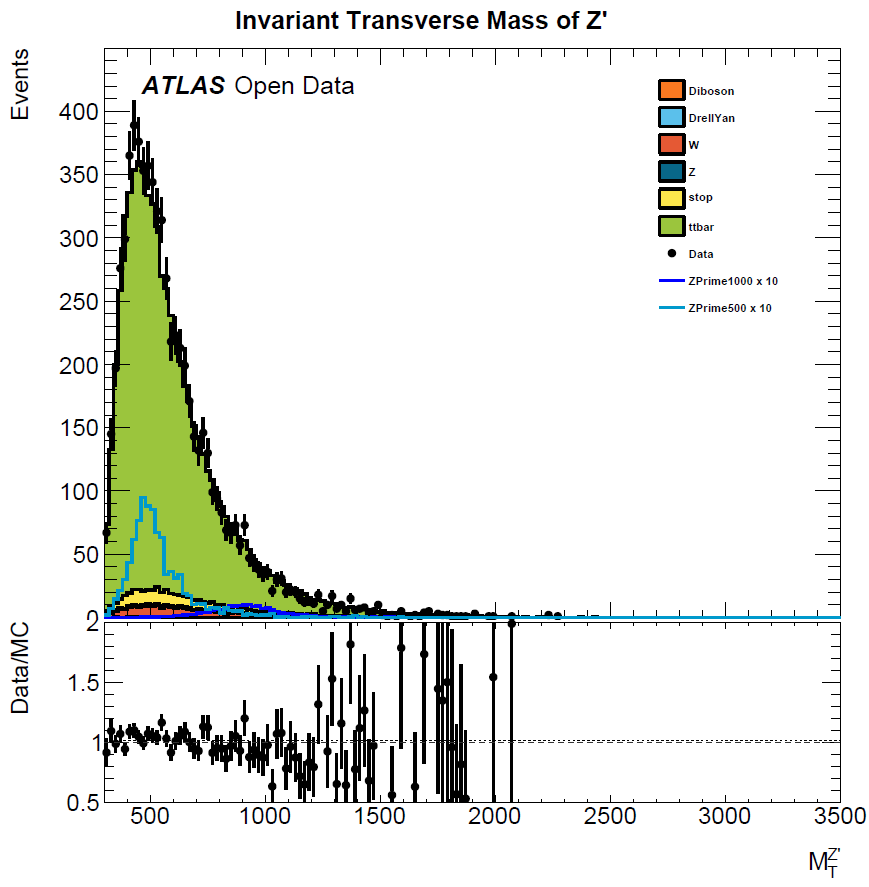
\includegraphics[width=.8\linewidth]{../Pictures/mass_before.png}
\caption{invariante Masse ohne Cuts}
\end{subfigure}%
\begin{subfigure}{.5\textwidth}
\centering
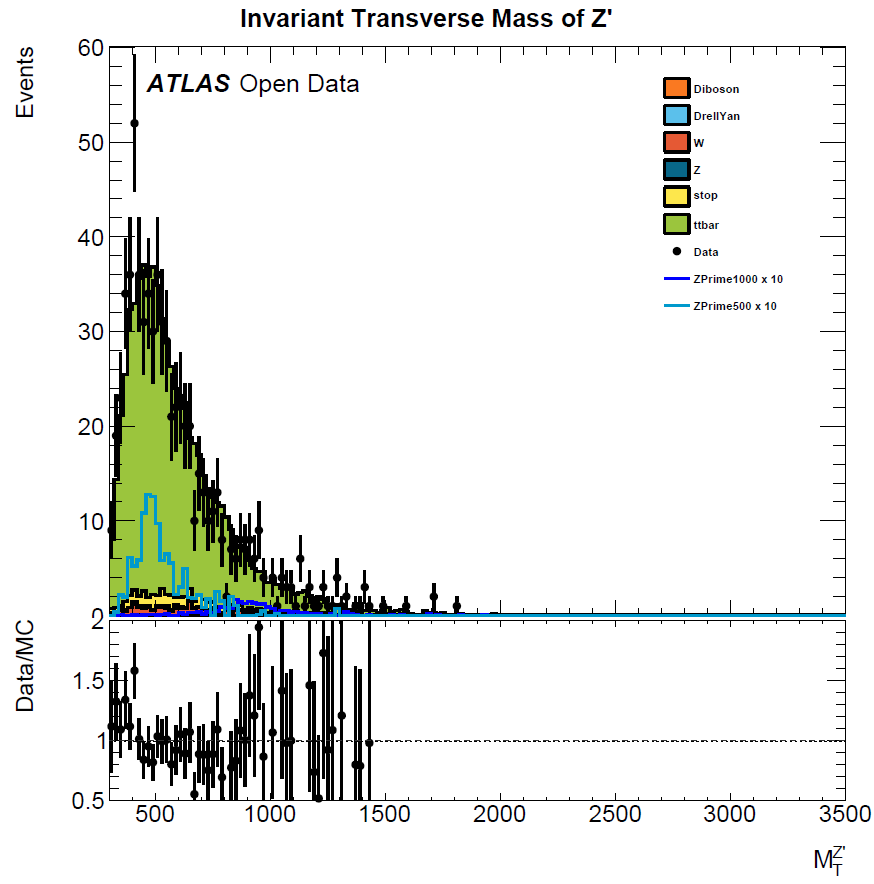
\includegraphics[width=.8\linewidth]{../Pictures/mass_after.png}
\caption{invariante Masse mit Cuts}
\end{subfigure}%
\caption{Auswirkungen der Cuts auf die Ereignisse }
\label{Cuts_z}
\end{figure}

Mit den so erhaltenen Daten wurden wieder p-Value Berechnungen für beide ausgewählte Massen durchgeführt.
Diesmal wurden für die Berechnungen jedoch nicht für das gesamte vorhandene Spektrum, sondern nur für den Bereich mit dem besten Verhältnis aus Signal und Untergrund genutzt.
Als Ergebnis ergaben sich folgende Werte:
\begin{center}
\begin{tabular}{c | c | c }
Masse [GeV] & p-Value & obere Grenze für $\mu$ \\
\hline
$400$ & 0,032 & 4,6 \\
$500$ & 0,11 & 5,2 \\
\end{tabular}
\end{center}
Alle anderen betrachteten Massehypothesen (bis zu $2500$ GeV) resultierten in p-Value Werten von $0,99...$ oder gar $1$, was sich so interpretieren lässt, dass die Daten perfekt ohne ein $Z'$ dieser Masse erklärt werden können.

Für die Interpretation erinnern wir uns an die Bedeutung des p-Values: Um von der Entdeckung eines neuen Teilchens zu reden, ist ein p-Value von $5,7 \cdot 10^{-7}$ notwendig.
Da unsere Werte deutlich höher sind, wurde also kein $Z'$-gefunden.
Ein Unterschreiten des p-Values von $0,05$ ($2 \sigma$) ist jedoch ausreichend um die Nullhypothese zu verwerfen.
Dies liegt offenbar für ein $Z'$ der Masse $400$ GeV vor.
Für die Masse von $500$ GeV wurde ein Wert von nur $0,11$ bestimmt, was für sich alleine gesehen mit hoher Wahrscheinlichkeit Rauschen entspricht.
In Kombination mit den deutlich besseren Wert für $400$ GeV kann dies jedoch als Indiz für ein Ereignis in diesem Massenbereich gesehen werden.
Dies wäre ausreichend um eine nähere Beschäftigung mit dem $Z'$ oder den Daten zu motivieren.

\clearpage